\documentclass[xetex,mathserif,serif]{beamer}

\usepackage{mathspec}
\usepackage{xltxtra,fontspec,xunicode}
\usepackage{listings}

% \usepackage{pgfpages}
% \pgfpagesuselayout{4 on 1}[a4paper,border shrink=5mm,landscape]

% Features
\setbeamertemplate{navigation symbols}{}

% Fonts
\setmainfont{Helvetica}
\setmathsfont(Digits,Latin,Greek){Helvetica}
\setmonofont{Monaco}

% Macros
\definecolor{CodeColor}{RGB}{0,112,0}
\newcommand{\code}[1]{\mbox{\texttt{\small{\color{CodeColor}{#1}}}}}

\title{Faster persistent data structures through hashing}
\author{Johan Tibell\\johan.tibell@gmail.com}
\date{2011-09-23}

\begin{document}
\lstset{
  language=Haskell,
  basicstyle=\small,
  keywordstyle=,
  commentstyle=\color{CodeColor}}

\frame{\titlepage}

\begin{frame}
  \frametitle{Motivating problem: Twitter data analys}

  ``I'm computing a communication graph from Twitter data and then
  scan it daily to allocate social capital to nodes behaving in a good
  karmic manner.  The graph is culled from 100 million tweets and has
  about 3 million nodes.''

  \bigskip
  We need a data structure that is
  \begin{itemize}
  \item fast when used with string keys, and
  \item doesn't use too much memory.
  \end{itemize}
\end{frame}

\begin{frame}
  \frametitle{Persistent maps in Haskell}

  \begin{itemize}
  \item \code{Data.Map} is the most commonly used map type.
  \item It's implemented using size balanced trees.
  \item Keys can be of any type, as long as values of the type can be
    ordered.
  \end{itemize}
\end{frame}

\begin{frame}
  \frametitle{Real world performance of Data.Map}

  \begin{itemize}
  \item Good in theory: no more than $O(\log n)$ comparisons.
  \item Not great in practice: up to $O(\log n)$ comparisons!
  \item Many common types are expensive to compare e.g
    \code{String}, \code{ByteString}, and \code{Text}.
  \item Given a string of length $k$, we need $O(k*\log n)$
    comparisons to look up an entry.
  \end{itemize}
\end{frame}

\begin{frame}
  \frametitle{Hash tables}
  \begin{itemize}
  \item Hash tables perform well with string keys: $O(k)$ amortized
    lookup time for strings of length $k$.
  \item However, we want persistent maps, not mutable hash tables.
  \end{itemize}
\end{frame}

\begin{frame}
  \frametitle{Milan Straka's idea: Patricia trees as sparse arrays}
  \begin{itemize}
  \item We can use hashing without using hash tables!
  \item A Patricia tree implements a persistent, sparse array.
  \item Patricia trees are as twice fast as size balanced trees, but
    only work with \code{Int} keys.
  \item Use hashing to derive an \code{Int} from an arbitrary
    key.
  \end{itemize}
\end{frame}

\begin{frame}
  \frametitle{Implementation tricks}
  \begin{itemize}
  \item Patricia trees implement a sparse, persistent array of size
    $2^{32}$ (or $2^{64}$).
  \item Hashing using this many buckets makes collisions rare: for
    $2^{24}$ entries we expect about 32,000 single collisions.
  \item Linked lists are a perfectly adequate collision resolution
    strategy.
  \end{itemize}
\end{frame}

\begin{frame}[fragile]
  \frametitle{First attempt at an implementation}
  \begin{lstlisting}
-- Defined in the containers package.
data IntMap a
    = Nil
    | Tip {-# UNPACK #-} !Key a
    | Bin {-# UNPACK #-} !Prefix
          {-# UNPACK #-} !Mask
          !(IntMap a) !(IntMap a)

type Prefix = Int
type Mask   = Int
type Key    = Int

newtype HashMap k v = HashMap (IntMap [(k, v)])
  \end{lstlisting}
\end{frame}


\begin{frame}[fragile]
  \frametitle{A more memory efficient implementation}
  \begin{lstlisting}
data HashMap k v
    = Nil
    | Tip {-# UNPACK #-} !Hash
          {-# UNPACK #-} !(FL.FullList k v)
    | Bin {-# UNPACK #-} !Prefix
          {-# UNPACK #-} !Mask
          !(HashMap k v) !(HashMap k v)

type Prefix = Int
type Mask   = Int
type Hash   = Int

data FullList k v = FL !k !v !(List k v)
data List k v = Nil | Cons !k !v !(List k v)
  \end{lstlisting}
\end{frame}

\begin{frame}
  \frametitle{Reducing the memory footprint}
  \begin{itemize}
  \item \code{List k v} uses 2 fewer words per key/value pair
    than \code{[(k, v)]}.
  \item \code{FullList} can be unpacked into the \code{Tip}
    constructor as it's a product type, saving 2 more words.
  \item Always unpack word sized types, like \code{Int}, unless
    you really need them to be lazy.
  \end{itemize}
\end{frame}

\begin{frame}
  \frametitle{Benchmarks}

  Keys: $2^{12}$ random 8-byte \code{ByteString}s

  \bigskip
  \begin{tabular}{|c|c|c|}
    \hline  & \textbf{Map} & \textbf{HashMap} \\
    \hline \textbf{insert} & 1.00 & 0.43 \\
    \hline \textbf{lookup} & 1.00 & 0.28 \\
    \hline
  \end{tabular}
  \bigskip

  \code{delete} performs like \code{insert}.
\end{frame}

\begin{frame}
  \frametitle{Can we do better?}
  \begin{itemize}
  \item We still need to perform $O(min(W, \log n))$ \code{Int}
    comparisons, where $W$ is the number of bits in a word.
  \item The memory overhead per key/value pair is still quite high.
  \end{itemize}
\end{frame}

\begin{frame}
  \frametitle{Borrowing from our neighbours}
  \begin{itemize}
  \item Clojure uses a \emph{hash-array mapped trie} (HAMT) data
    structure to implement persistent maps.
  \item Described in the paper ``Ideal Hash Trees'' by Bagwell (2001).
  \item Originally a mutable data structure implemented in C++.
  \item Clojure's persistent version was created by Rich Hickey.
  \end{itemize}
\end{frame}

\begin{frame}
  \frametitle{Hash-array mapped tries in Clojure}
  \begin{itemize}
  \item Shallow tree with high branching factor.
  \item Each node, except the leaf nodes, contains an array of up to
    32 elements.
  \item 5 bits of the hash are used to index the array at each level.
  \item A clever trick, using bit population count, is used to
    represent sparse arrays.
  \end{itemize}
\end{frame}

\begin{frame}[fragile]
  \frametitle{The Haskell definition of a HAMT}
  \begin{lstlisting}
data HashMap k v
    = Empty
    | BitmapIndexed
          {-# UNPACK #-} !Bitmap
          {-# UNPACK #-} !(Array (HashMap k v))
    | Leaf {-# UNPACK #-} !(Leaf k v)
    | Full {-# UNPACK #-} !(Array (HashMap k v))
    | Collision {-# UNPACK #-} !Hash
                {-# UNPACK #-} !(Array (Leaf k v))

type Bitmap = Word

data Array a = Array !(Array# a)
                     {-# UNPACK #-} !Int
  \end{lstlisting}
\end{frame}

\begin{frame}
  \frametitle{Making it fast}
  \begin{itemize}
  \item The initial implementation by Edward Z. Yang: correct but
    didn't perform well.
    \item Improved performance by
      \begin{itemize}
        \item replacing use of \code{Data.Vector} by a
          specialized array type,
        \item paying careful attention to strictness, and
        \item using GHC's new \code{INLINABLE} pragma.
      \end{itemize}
  \end{itemize}
\end{frame}

\begin{frame}
  \frametitle{Benchmarks}

  Keys: $2^{12}$ random 8-byte \code{ByteString}s

  \bigskip
  \begin{tabular}{|c|c|c|c|}
    \hline  & \textbf{Map} & \textbf{HashMap} &
    \textbf{HashMap (HAMT)} \\
    \hline \textbf{insert} & 1.00 & 0.43 & 1.21 \\
    \hline \textbf{lookup} & 1.00 & 0.28 & 0.21 \\
    \hline
  \end{tabular}
\end{frame}

\begin{frame}
  \frametitle{Where is all the time spent?}

  \begin{itemize}
  \item Most time in \code{insert} is spent copying small arrays.
  \item Array copying is implemented using \code{indexArray\#}
    and \code{writeArray\#}, which results in poor performance.
  \item When cloning an array, we are force to first fill the new
    array with dummy elements, followed by copying over the elements
    from the old array.
  \end{itemize}
\end{frame}

\begin{frame}
  \frametitle{A better array copy}

  \begin{itemize}
  \item Daniel Peebles have implemented a set of new primops for
    copying array in GHC.
  \item The first implementation showed a 20\% performance improvement
    for \code{insert}.
  \item Copying arrays is still slow so there might be room for big
    improvements still.
  \end{itemize}
\end{frame}

\begin{frame}
  \frametitle{Other possible performance improvements}
  \begin{itemize}
  \item Even faster array copying using SSE instructions, inline
    memory allocation, and C-- inlining.
  \item Use dedicated bit population count instruction on
    architectures where it's available.
  \item Clojure uses a clever trick to unpack keys and values directly
    into the arrays; keys are stored at even positions and values at
    odd positions.
  \item GHC 7.2 will use 1 less word for \code{Array}.
  \end{itemize}
\end{frame}

\begin{frame}
  \frametitle{Optimize common cases}
  \begin{itemize}
  \item In many cases maps are created in one go from a sequence of
    key/value pairs.
  \item We can optimize for this case by repeatedly mutating the HAMT
    and freeze it when we're done.
  \end{itemize}

  \bigskip
  Keys: $2^{12}$ random 8-byte \code{ByteString}s

  \bigskip
  \begin{tabular}{|c|c|}
    \hline \textbf{fromList/pure} & 1.00 \\
    \hline \textbf{fromList/mutating} & 0.50 \\
    \hline
  \end{tabular}
\end{frame}

\begin{frame}
  \frametitle{Abstracting over collection types}
  \begin{itemize}
  \item We will soon have two map types worth using (one ordered and one
    unordered).
  \item We want to write functions that work with both types, without a
    $O(n)$ conversion cost.
  \item Use type families to abstract over different concrete
    implementations.
  \end{itemize}
\end{frame}

\begin{frame}
  \frametitle{Summary}
  \begin{itemize}
  \item Hashing allows us to create more efficient data structures.
  \item There are new interesting data structures out there that have,
    or could have, an efficient persistent implementation.
  \end{itemize}
\end{frame}

\begin{frame}
  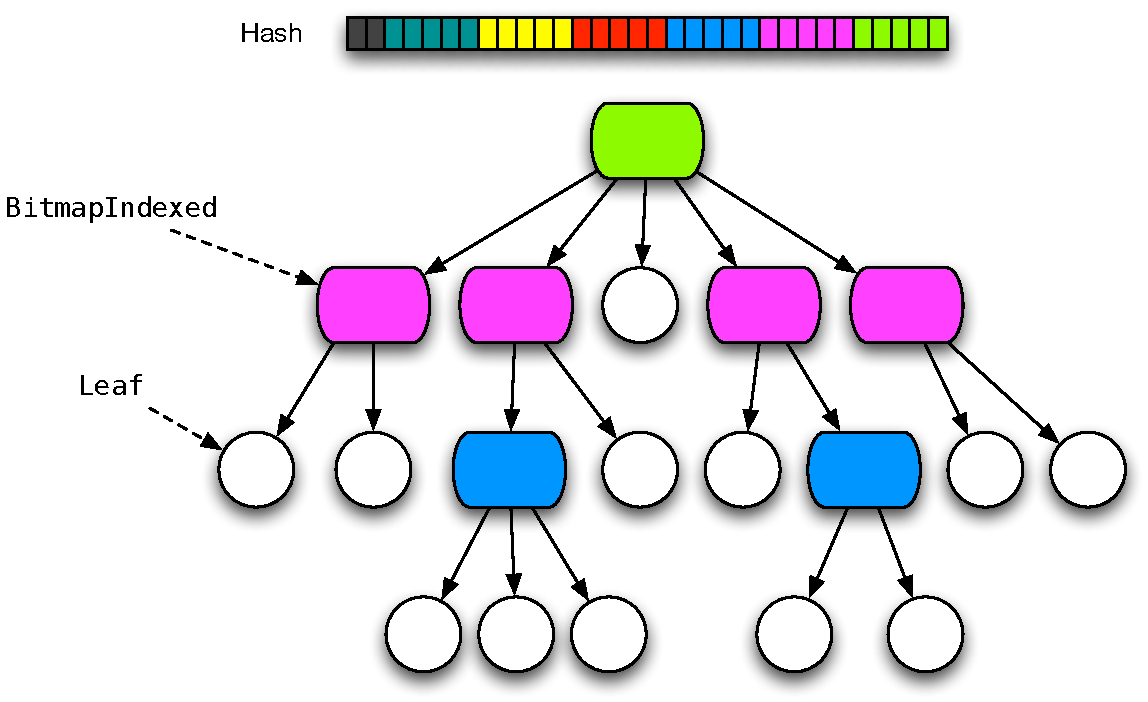
\includegraphics[width=\textwidth]{hamt.pdf}
\end{frame}

\end{document}

%%% Local Variables:
%%% mode: latex
%%% TeX-master: t
%%% TeX-PDF-mode: t
%%% End:
